% !TeX spellcheck = ru_RU
% !TEX root=../main.tex

\begin{lecture}[Потенциал Гиббса]
	
	\begin{lecSection}[Термодинамические потенциалы]
	Термодинамические потенциалы:
	\begin{equation}	
	\begin{aligned}
	U = U(S,V) \tab H = H(S,P) \tab F = F(T,V) \tab G = G(T,P)
	\end{aligned}
	\end{equation}
	
	Параметры $T,p$ удобны для измерений.
	
	\begin{definition}
		Химический потенциал: $\mu_i = \left( \dfrac{\partial G}{\partial n_i} \right)_{p, T, n_j (j \neq i)}$
	\end{definition}
	
	При этом $G = \sum\limits_{i=1}^{N} \mu_i n_i$, где $n_i$ - концентрация.
	
	\begin{definition}
		Супрамолекулярные системы --- это системы, образующиеся за счет слабых межмолекулярных взаимодействий.
	\end{definition}
	
	Любое самопроизвольное изменение в системе происходит с уменьшением энергии Гиббса: $(dG)_{p,T}\geq0$.
	\begin{wrapfigure}[6]{l}{0.23\linewidth}
		\centering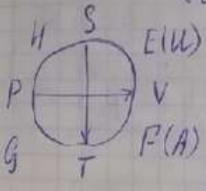
\includegraphics[width=\linewidth]{lecture_02/pic1}
	\end{wrapfigure}
	\nobreak
	
	\begin{align}
	G = G(p,T) \\
	dG = Vdp - SdT
	\end{align}
	
	\begin{center}
		\textbf{Единицы измерения}\\
	\end{center}
	
	\begin{itemize}
		\item молярность $[C] = \frac{\text{моль}}{\text{л}} = M$
		\item моляльность $[C] = \frac{\text{кол-во моль растворенного в-ва}}{\text{1000 г растворителя}}$
		\item мольная доля $\chi_i = \frac{n_i}{\sum\limits_{j=1} n_j}, n_i $ - количество молей
		\item 1 кал $\simeq 4$ Дж, 1 Дж $= 10^7$ эрг
		\item 1 эВ $\simeq 23 \frac{\text{ккал}}{\text{моль}}$
		\item $kT \simeq \frac{1}{40}$ эВ
	\end{itemize}
	
	\begin{center}
		\textbf{Некоторые константы}\\
	\end{center}
	
	\begin{itemize}
		\item $N_A \simeq 6 \cdot 10^{23} \frac{1}{\text{моль}}$
		\item $k_{\text{Б}} = 1,4 \cdot 10^{-16} \frac{\text{эрг}}{\text{град}}$
		\item $e = 4,8 \cdot 10^{-10}$ ед. СГСЭ
		\item $Rg = \frac{e^2}{2r} \simeq 13,6$ эВ
	\end{itemize}
	\end{lecSection}

	\begin{lecSection}[Соотношения Гиббса-Гельмольца]

	
	\begin{equation}	
	\begin{aligned}
	G = H - TS \tab dG = -SdT + Vdp \tab S = - \left( \dfrac{\partial G}{\partial T} \right)_{p}
	\end{aligned}
	\end{equation}
	
	\begin{equation}
	H = G - T\left( \dfrac{\partial G}{\partial T} \right)_{p} = -T^2 \left(\left[\frac{1}{T}\left( \dfrac{\partial G}{\partial T} \right)_{p}\right] - \frac{1}{T^2}G\right) = -T^2 \left[\dfrac{\partial}{\partial T}\left(\frac{G}{T}\right)\right]
	\end{equation}
	
	\begin{equation}	
	\begin{aligned}
	\Delta H = Q_p \tab -\Delta G = A_{max} \tab G = T \int H d \left( \frac{1}{T}\right)
	\end{aligned}
	\end{equation}
	
	\end{lecSection}

	\begin{lecSection}[Пример]

	\begin{equation}
	\mathrm{N_2 + 3H_2 \rightleftharpoons  2NH_3}
	\end{equation}
	
	Степень протекания реакции(пробег реакции): $\xi$.
	\begin{equation}	
	\begin{aligned}
	d \xi = \frac{dn_i}{\nu_i} \tab d\xi = \frac{dn_{\mathrm{NH_3}}}{2} = -dn_{\mathrm{N_2}} = -\frac{dn_{\mathrm{H_2}}}{3}
	\end{aligned}
	\end{equation}	
	
	Общий вид реакции: $\sum\limits_{i} \nu_i A_i = \sum\limits_{j} \nu_j A_j$
	
	\begin{equation}
	dG = -SdT + Vdp - \mu_1dn_1 - \mu_2dn_2 - ... + \mu_1'dn_1' + \mu_2'dn_2' + ...  
	\end{equation}
	
	\begin{equation}
	dG = -SdT + Vdp - \mu_1\nu_1d\xi - \mu_2\nu_2d\xi - ... + \mu_1'\nu_1'd\xi + \mu_2'\nu_2'd\xi + ...
	\end{equation}
	
	\begin{equation}
	T,p = const \Rightarrow dG = (\sum\limits_{j} \nu_j'\mu_j' - \sum\limits_{i} \nu_i\mu_i) d \xi
	\end{equation}
	\par $\left( \dfrac{\partial G}{\partial \xi} \right)_{p,T} = 0$ в равновесии. Итого: $(\sum\limits_{j} \nu_j'\mu_j' - \sum\limits_{i} \nu_i\mu_i) = 0$
	\begin{wrapfigure}{l}{0.3\linewidth}
		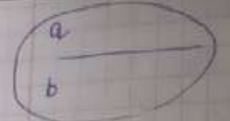
\includegraphics[width=\linewidth]{lecture_02/pic2}
	\end{wrapfigure}
	
	\par Пусть молекулы вещества переходят из части а в часть b. 
	
	\begin{equation}	
	\begin{aligned}
	dG = \mu^a_idn^a_i + \mu^b_idn^b_i \tab n^a_i+n^b_i = n = const \tab dn^a_i = -dn^b_i
	\end{aligned}
	\end{equation}
	
	$dG = (\mu^a_i - \mu^b_i) dn^a_i, \mu^a_i > \mu^b_i \Rightarrow $ процесс идет в направлении $a \rightarrow b$. Равновесие достигается при $\mu^a_i = \mu^b_i$.
	\par Рассмотрим идеальный газ:
	\begin{equation}	
	\begin{aligned}
	\left(\dfrac{\partial \mu_i}{\partial p}\right)_T = v_i \tab pv_i = RT \tab \left(\dfrac{\partial \mu_i}{\partial p}\right)_T = \frac{RT}{p} \rightarrow \mu_i - \mu_i^0 = RT \text{ ln} \frac{p}{p_0} 
	\end{aligned}
	\end{equation}
	В приближении идеального газа: $\mu_i = \mu_i^0 + RT \text{ ln} n_i$, где $\mu_i^0$ - стандартный химический потенциал. Это выражение верно для газа и конденсированных сред, когда концентрации малы.
\end{lecSection}

	
\end{lecture}
